In this chapter, the requirements of a system that can solve the problem described in the problem definition \ref{problemdefinition} has been defined. This has been done by first describing different use cases for the system and then analyzing them to get a formal list of requirements.

\section{System behaviour}
To better understand how the system of this report could work, this section contains a more in-depth description of an actual situation we imagine the system being used in. This includes descriptions of how each part of the system should respond to an event.

The system should be activated upon one of the following conditions, that triggers during or after the falling accident has happened:

\begin{itemize}
    \item The smartphone detects a falling event
    \item The personal assistant detects a falling event
\end{itemize}

\begin{figure}[H]
    \centering
    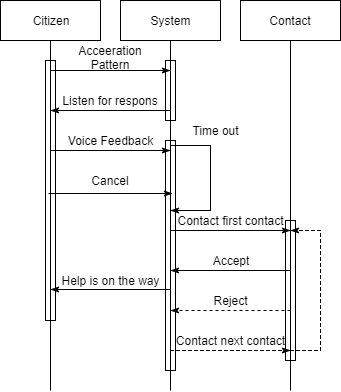
\includegraphics[width=0.7\textwidth]{Figures/Phone.png}
    \caption{Sequence diagram for smartphone app}
    \label{fig:SmartPhoneApp}
\end{figure}

When the smartphone detects a falling event, it should wait a short while for user response, either in the form of a button-press or voice-detection. This would allow for the user to interrupt the process, and therefore avoid emergency services or contact person being contacted when they are not needed. When a short while has passed, and no user interaction has happened, it should begin to contact people from that citizen contact list in the priorities order, this can be seen in the graph \ref{fig:SmartPhoneApp}.

%Furthermore it should try and distinguish between false positives when detecting events. 

\begin{figure}[H]
    \centering
    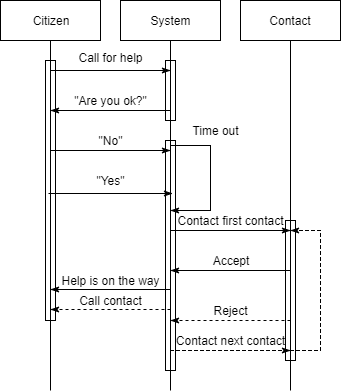
\includegraphics[width=0.7\textwidth]{Figures/PersonAssitent.png}
    \caption{Sequence diagram for personal assistant}
    \label{fig:PersonAssitent}
\end{figure}

When the personal assistant detects a falling accident it should verify that a falling accident has actually taken place, and then it notifies the system that the citizen has fallen and calls for help. The personal assistant receives confirmation that help has been requested and who have responded to it. The personal assistant should be context aware, so that it doesn't call for help during normal dialogue, and in general try to distinguish between false positives.

When the system gets an alert of a falling event it looks up the citizen in need of help, and find their contact list. It then tries to contact people on the contact list until someone on the list responds to the call for help. It should also be an option to call emergency services, if nobody on the contact list responds, this can be seen in \ref{fig:SmartPhoneApp} and \ref{fig:PersonAssitent} in the interaction between the system and contacts.

A contact receives a notification when the contact is the next person on the contact list. If the contact does not answer, the system will leave a message letting the contact know that an event has occurred. If they do answer, they can let the system know if they are able to help or not, and if they say they are currently unable to help, the system will treat it as a failed attempt to contact.

Apart from the above behaviours, the system should behave as follows when configuring new users and devices:

The new user must be configured through the web-interface. When they are added, it is necessary to include enough information so that it is possible for contacts to be identified. A contact list is created, the system should contact after a fall accident can be added. The contacts are prioritized, and will be contacted in the specified order when a falling accident happens. 

A new fall-detection device should be configured for the user, but it is not required that the user has a device.
The new device can possibly be an app for a smartphone, a voice-assistant configured for fall-detection, or other IoT enabled devices. These devices are coupled with a specific user upon configuration.

\subsection{Quantitative requirements}
To be able to validate the system later, it is important to define some quantitative values that later can be measured and compared to validate whether or not the system lives up to the requirements. Two values that can be defined are the amount of false positives allowed and the amount of false negatives allowed. 

A false positive is when the system registers a fall accident and sends out an alarm, when the citizen has not fallen. A false negative is when the system fails to register that a citizen has fallen.

\todo{hvor kommer 1 procent fra}
False negatives can have severe consequences for the user and must there for be avoided if at all possible. To perceive the system as a success it cannot have more than 1\% falls negatives. To be able to adhere to this low tolerance, the system might make more falls positives than with a higher fault tolerance for false negatives, since it will have to send out an alarm when it might not be needed, for example in cases where no input is giving to the device after an acceleration.

\todo{bindetekst}
The solution \textit{Lifeline} \cite{AAlert}, claims that they have an accuracy of 95\%, meaning that 5\% of their alarms are false positive. For our system to do better, it would need to have an accuracy of 95\% or higher.


\section{MoSCoW analysis}
The functional requirements define the functionality of the system. To be able to prioritize the requirements, a MoSCoW analysis has been made, the result of which can be found below. \todo{below? Referer eller henvis til noget ala "this section"}

\subsection{Must have}

\begin{itemize}
    \item Functionality to add and administrate citizens without need for a system administrator.
    \item Detect when a citizen has had a fall accident, through input from the user on a device, such as a smartphone or wearable.
    \item Send an alarm to a prioritized list of contact persons, until someone reacts.
\end{itemize}

\subsection{Should have}

\begin{itemize}
    \item Detect when a citizen has had a fall accident, through conversation with a personal assistant.
\end{itemize}

\subsection{Could have}
\begin{itemize}
    \item Be able to integrate IoT devices and wearable tech such as actuators and sensors.
        \begin{itemize}
            \item Associate device with a citizen to send alarms using device.
            \item Associate device with a contact person to receive alarms using device.
        \end{itemize}
\end{itemize}

\subsection{Won't have}

We have marked the following items for wont have, since we do not have the time to complete these tasks before the deadline.
\begin{itemize}
    \item Automatically detect when a citizen has had a fall accident, using a smartphone.
    \item Have a high accuracy when detecting a fall accident.
    \begin{itemize}
        \item No more than 5\% false positives.
        \item No more than 1\% false negatives.
    \end{itemize}
\end{itemize}



% The following items have yet to be added to the moscow analysis
\begin{itemize}
    



    

    

    
    \item Facilitate communication between a citizen and contact person during a fall accident.


    

    
    
\end{itemize}

%This chapter has described the requirements for the finished system, that we will use to verify later in the report.
%\todo{omg dis is so bad}

%The requirements stated above, presents the FUCK IT IM OUT!



\todo{Outro}